\documentclass{article} % For LaTeX2e
\usepackage{nips14submit_e,times}
\usepackage{amsmath}
\usepackage{amsthm}
\usepackage{amssymb}
\usepackage{mathtools}
\usepackage{hyperref}
\usepackage{url}
\usepackage{algorithm}
\usepackage[noend]{algpseudocode}
%\documentstyle[nips14submit_09,times,art10]{article} % For LaTeX 2.09

\usepackage{graphicx}
\usepackage{caption}
\usepackage{subcaption}

\def\eQb#1\eQe{\begin{eqnarray*}#1\end{eqnarray*}}
\def\eQnb#1\eQne{\begin{eqnarray}#1\end{eqnarray}}
\providecommand{\e}[1]{\ensuremath{\times 10^{#1}}}
\providecommand{\pb}[0]{\pagebreak}

\newcommand{\E}{\mathrm{E}}
\newcommand{\Var}{\mathrm{Var}}
\newcommand{\Cov}{\mathrm{Cov}}

\def\Qb#1\Qe{\begin{question}#1\end{question}}
\def\Sb#1\Se{\begin{solution}#1\end{solution}}

\newenvironment{claim}[1]{\par\noindent\underline{Claim:}\space#1}{}
\newtheoremstyle{quest}{\topsep}{\topsep}{}{}{\bfseries}{}{ }{\thmname{#1}\thmnote{ #3}.}
\theoremstyle{quest}
\newtheorem*{definition}{Definition}
\newtheorem*{theorem}{Theorem}
\newtheorem*{lemma}{Lemma}
\newtheorem*{question}{Question}
\newtheorem*{preposition}{Preposition}
\newtheorem*{exercise}{Exercise}
\newtheorem*{challengeproblem}{Challenge Problem}
\newtheorem*{solution}{Solution}
\newtheorem*{remark}{Remark}
\usepackage{verbatimbox}
\usepackage{listings}
\title{Complex Analysis I: \\
Problem Set IX}


\author{
Youngduck Choi \\
CILVR Lab \\
New York University\\
\texttt{yc1104@nyu.edu} \\
}


% The \author macro works with any number of authors. There are two commands
% used to separate the names and addresses of multiple authors: \And and \AND.
%
% Using \And between authors leaves it to \LaTeX{} to determine where to break
% the lines. Using \AND forces a linebreak at that point. So, if \LaTeX{}
% puts 3 of 4 authors names on the first line, and the last on the second
% line, try using \AND instead of \And before the third author name.

\newcommand{\fix}{\marginpar{FIX}}
\newcommand{\new}{\marginpar{NEW}}

\nipsfinalcopy % Uncomment for camera-ready version

\begin{document}


\maketitle

\begin{abstract}
This work contains the solutions to the problem set IX
of Complex Analysis I 2015 at Courant Institute of Mathematical Sciences.
\end{abstract}

\bigskip

\begin{question}[1]
\hfill
\begin{figure}[h!]
\centering
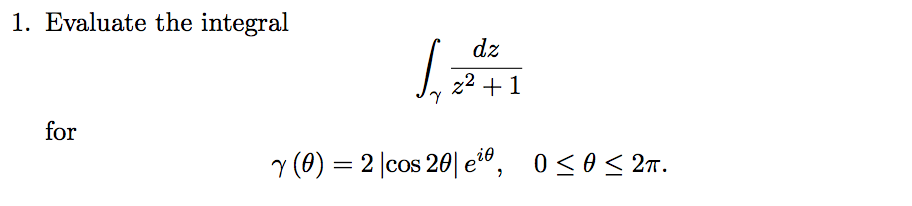
\includegraphics[width=1\textwidth]{cv-9-1}
\end{figure}
\end{question}
\begin{solution}
By drawing the contour on the complex plane, we observe that 
$\gamma$ forms 4 simple closed contours, for each direction of the axis.
We denote these contours as $\gamma_1$, $\gamma_2$, $\gamma_3$, and
$\gamma_4$ respectively in a counter-clockwise fashion. Observe that
$f(z) = \dfrac{1}{z^2+1}$ is singular at $z = \pm i$. $z = i$ belongs
to the interior of $\gamma_2$ contour, and $z = -i$ belongs to the
interior of $\gamma_4$ contour. By the Cauchy-Residue formula, we obtain
\eQb
\int_{\gamma_1} \dfrac{dz}{z^2+1} &=& 0 \\
\int_{\gamma_2} \dfrac{dz}{z^2+1} &=& 2\pi i 
\text{Res}_{z=i} \dfrac{1}{z^2+1}  \\
\int_{\gamma_3} \dfrac{dz}{z^2+1} &=& 0 \\
\int_{\gamma_4} \dfrac{dz}{z^2+1} &=& 2\pi i 
\text{Res}_{z=-i} \dfrac{1}{z^2+1}.\\
\eQe
As it can be written that
$f(z) = \dfrac{\phi(z)}{z-i}$, where $\phi(z) = \dfrac{1}{z+i}$,
the residue at $z = i$ is $\phi(i) = \dfrac{1}{2i}$. On the other hand,
as it can be written that
$f(z) = \dfrac{\phi(z)}{z+i}$, where $\phi(z) = \dfrac{1}{z-i}$, 
the residue at $z = -i$ is $\phi(i) = -\dfrac{1}{2i}$. Consequently, we have
\eQb
\int_{\gamma_2} \dfrac{dz}{z^2+1} &=& 2\pi i \dfrac{1}{2i} = \pi  \\
\int_{\gamma_4} \dfrac{dz}{z^2+1} &=& 2\pi i (-\dfrac{1}{2i}) = -\pi. \\
\eQe
Therefore, it follows that
\eQb
\int_{\gamma} \dfrac{dz}{z^2+1} &=& 
\int_{\gamma_1} \dfrac{dz}{z^2+1} + 
\int_{\gamma_2} \dfrac{dz}{z^2+1} +
\int_{\gamma_3} \dfrac{dz}{z^2+1} +
\int_{\gamma_4} \dfrac{dz}{z^2+1} \\
&=& 0.
\eQe
\hfill $\qed$
\end{solution}

\bigskip
\begin{question}[2]
\hfill
\begin{figure}[h!]
\centering
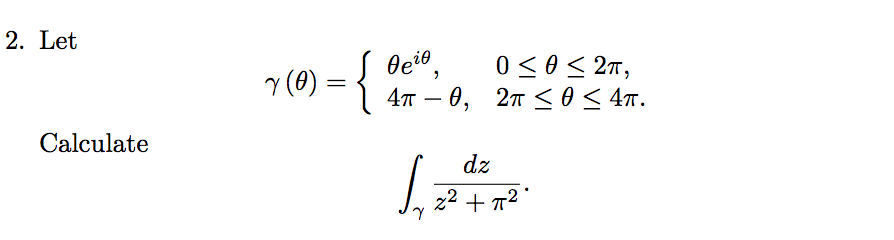
\includegraphics[width=1\textwidth]{cv-9-2}
\end{figure}
\end{question}
\begin{solution}
Observe that the function has isolated singularities at $z = \pm i \pi$. 
By observing the contour, we see that $i \pi$ lies outside of the contour,
as $\gamma(\dfrac{\pi}{2}) = \dfrac{\pi}{2}e^{i\frac{\pi}{2}} = 
i\dfrac{\pi}{2}$. On the other hand, $z = -i\pi$ lies on the interior of the
contour 
as $\gamma(\dfrac{3\pi}{2}) = \dfrac{3\pi}{2}e^{i\frac{3\pi}{2}} =
-\dfrac{3\pi}{2}i$. Hence, by the Cauchy Residue theorem, we have
\eQb
\int_{\gamma} \dfrac{dz}{z^2+\pi^2} &=& 2\pi i \text{Res}_{z=-i\pi} 
\dfrac{1}{z^2+\pi^2}.
\eQe  
As it can be written that $f(z) = \dfrac{\phi(z)}{z+i\pi}$, where
$\phi(z) = \dfrac{1}{z - i\pi}$, the residue at $z=-i\pi$ is 
$\phi(-i\pi) = -\dfrac{1}{2i\pi}$. Hence, it follows that
\eQb
\int_{\gamma} \dfrac{dz}{z^2+\pi^2} &=& 2\pi i (-\dfrac{1}{2i\pi}) \\
&=& -1. 
\eQe
\hfill $\qed$
\end{solution}

\newpage

\begin{question}[3]
\hfill
\begin{figure}[h!]
\centering
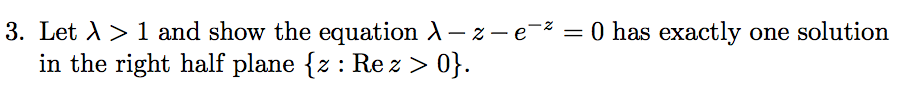
\includegraphics[width=1\textwidth]{cv-9-3}
\end{figure}
\end{question}
\begin{solution}
Firstly, the equation can be re-written as $\lambda - z = e^{z}$.
Observe that it is necessary to have
$| \lambda - z | = e^{-\text{Re} z}$ to satisfy the above equation.
As we only limit the space of possible solutions to be $\{ z : \text{Re} z 
> 0\}$, it follows that it is necessary to have $|\lambda - z | < 1$.
Define $C = \{ z \in \mathbb{C} \> | \> | \lambda - z| < 1 \}$. So far,
we have shown that the solutions to the given equation, if it exists
must lie on the interior of $C$. 
Let $f(z) = e^{-z}$
and $g(z) = \lambda - z $. Then, it follows that on $C$, $|g(z)| = |\lambda
-z | = 1$, and as $\lambda > 1$, $|f(z)| = |e^{-z}| = e^{-\text{Re}z} < 1$. 
As $f(z)$ and $g(z)$ are entire, they are also analytic inside
and on $C$. The conditions of Rouche's theorem are thus satisfied. Hence,
$\lambda - z$ and $\lambda - z - e^{-z}$ have the same number of zeros, 
counting multiplicities inside $C$. Observe that $\lambda - z$ has a 
zero on $z = \lambda$. Thus, $\lambda -z -e^{-z}$ has one solution
inside $C$. As we have shown that a solution to $\lambda -z -e^{-\lambda}$
must lie inside $C$, we have shown that $\lambda -z -e^{\lambda}$ has
exactly one solution. \hfill $\qed$

\end{solution}

\bigskip

\begin{question}[4]
\hfill
\begin{figure}[h!]
\centering
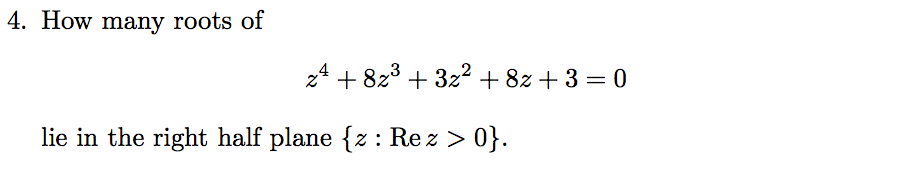
\includegraphics[width=1\textwidth]{cv-9-4}
\end{figure}
\end{question}
\begin{solution}
Let $\gamma$ be a contour, which moves from $-iR$ to $iR$ as a semi-circle
of a radius $R$. On $\gamma$, we can parametrize $z$ has $z = Re^{i\theta}$.
Then, the given equation can be re-written as 
\eQb
R^{4}e^{i4\theta} (1 + \dfrac{8}{Re^{i\theta}} + 
\dfrac{3}{R^{2}e^{i2\theta}} + \dfrac{8}{R^{3}e^{i3\theta}}+ 
\dfrac{3}{R^{4}e^{i4\theta}}) &=& 0. \\
\eQe 
Observe that as $R \to \infty$, LHS $\to R^4e^{i4t}$. 
\end{solution}

\newpage

\begin{question}[5]
\hfill
\begin{figure}[h!]
\centering
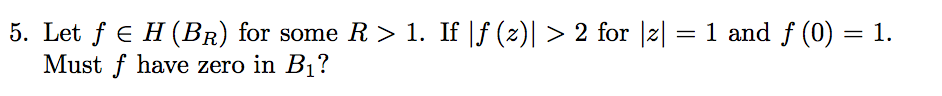
\includegraphics[width=1\textwidth]{cv-9-5}
\end{figure}
\end{question}
\begin{solution}
As $B_1$ is a circle of radius $1$, centered around the origin,
we have that the winding number of $B_1$ is simply $1$. Observe that
the given function is holomorphic, hence meromorphic with zero poles, 
interior to $B_1$ and is analytic on $B_1$. Furthermore, as $|f(z)| > 2$
for $|z| = 1$, we have $f$ is nonzero on $B_1$. Therefore, by the argument
principle, we have that the winding number is equal to $Z - P$ where
$Z$ is the number of zeros and $P$ is the number of poles of $f(z)$
inside $B_1$. Since $P = 0$ and the winding number is $1$,
 we have that $Z = 1$. $f$ must have zero in $B_1$.
 \hfill $\qed$
\end{solution}

\bigskip

\begin{question}[6]
\hfill
\begin{figure}[h!]
\centering
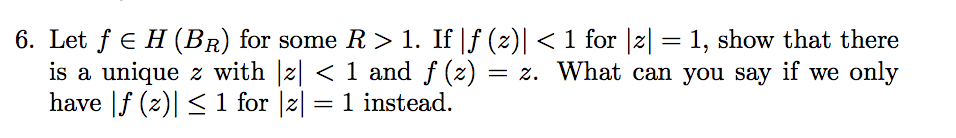
\includegraphics[width=1\textwidth]{cv-9-6}
\end{figure}
\end{question}
\begin{solution}
As $B_1$ is a circle of radius 1, centered around the origin, we
have that the winding number of $B_1$ is simply $1$. As $f$ is holomorphic
on $B_R$ for some $R > 1$, we have $f$ is analytic on $B_1$. On $B_1$, as 
we have $|f(z)| < 1$, it follows that 
$|f(z) - z| \leq ||f(z)| - |z|| = 1 - |f(z)| > 0$. Therefore, $f(z) - z$
is nonzero on $B_1$. Therefore, by the argument principle, as above,
with $P = 0$, we have $Z = 1$. Therefore, there exists a unique solution 
to the equation $f(z) - z = 0$ inside $B_1$, 
which is also a solution to $f(z) = z$ as well.
Hence, there exists a unique solution to $f(z) = z$ inside $B_1$. When
we only have $|f(z) \leq 1$ for $|z|| = 1$, we lose the nonzero property
of $f(z) - z$ on $B_1$. Therefore, the argument will not work in that case.
\hfill $\qed$
\end{solution}

\bigskip

\begin{question}[7]
\hfill
\begin{figure}[h!]
\centering
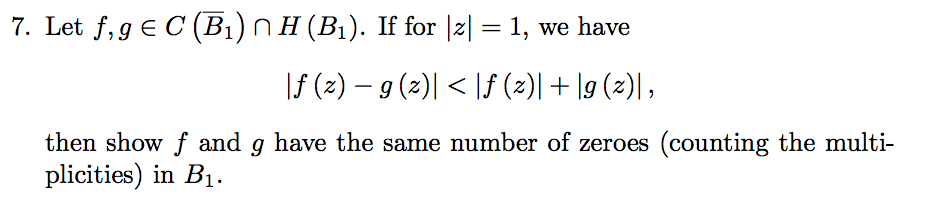
\includegraphics[width=1\textwidth]{cv-9-7}
\end{figure}
\end{question}
\begin{solution}
We are given that $f,g \in H(B_1)$ and $f,g$ are continuous on $B_1$. 
The conditions of symmetric Rouche's theorem are satisfied.
Then, by the Symmetric Rouche's theorem. we have the same number of
roots for $f$ and $g$, counting the multiplicies in $B_1$. 
\hfill $\qed$
\end{solution}


\end{document}


